%
% CMPT 379: Principles of Compiler Design - A Course Overview
% Section: Semantic Analysis and Static Single Assignment
%
% Author: Jeffrey Leung
%

\section{Semantic Analysis and Static Single Assignment}
	\label{sec:semantic-analysis-ssa}
\begin{easylist}

& \textbf{Semantic analysis:} Validating a program's basic requirements and type compatibilities, processing static semantic checks, and adding run-time semantic checks
	&& E.g. Checking that a \textit{main} function exists, that variables are declared, whether operand types are compatible

& \textbf{Static Single Assignment (SSA):} Property of an intermediate representation where each variable is only assigned once
	&& Used to distinguish and merge values from multiple possible paths of computation to create a single resulting value

& \textbf{Dominance:} Characteristic of a node which is a mandatory predecessor of another node (i.e. any path from the root to the lower node must pass through the upper node)
	&& Any node dominates itself
	&& Definitions of a variable dominate its later usages
	&& \textbf{Strict dominance:} Characteristic of a node which dominates a different node

& \textbf{Dominance Frontier (DF):} Set of nodes which, given a target node, are the convergence of two nodes - one which is dominated by the target node and one which is not (i.e. all nodes such that the target node dominates a predecessor but not the node itself)
	&& Notation: $DF(X)$
	&& Can include the node itself
	&& E.g. See figure~\ref{fig:dominance-frontier-example} which calculates the dominance frontier of node 5

\begin{figure}[!htb]
	\caption{Dominance Frontier Example}
	\label{fig:dominance-frontier-example}
	\begin{center}
		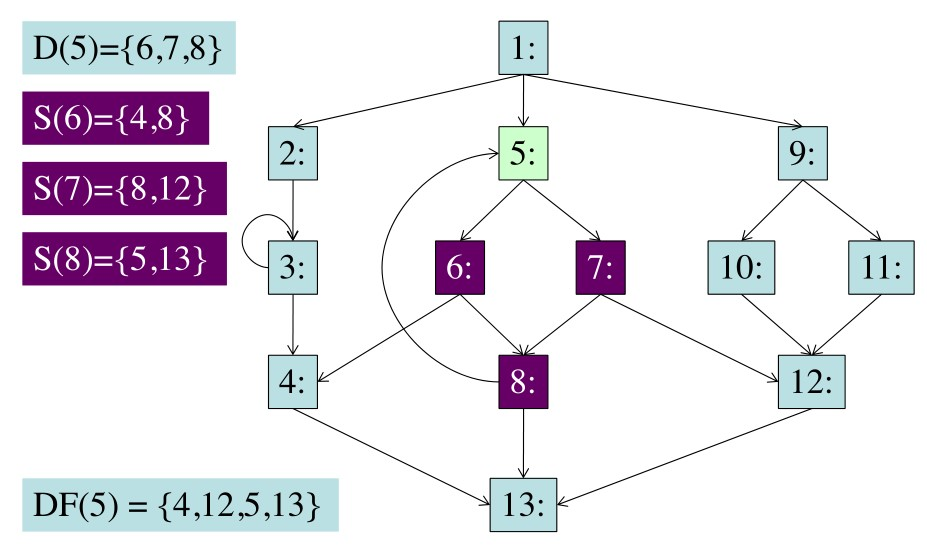
\includegraphics[width=\textwidth]{dominance-frontier}
	\end{center}
\end{figure}

	&& Every node in $DF(X)$ requires a $\phi$ (phi) function for each variable defined in $X$

& \textbf{Dominator tree:} Acyclical hierarchical structure of a set of nodes, where a node dominates all of its children

\end{easylist}
\clearpage
